\documentclass{aifyp}
\usepackage{lmodern}
\usepackage{float}

\usepackage{graphicx}
\usepackage[bottom]{footmisc}
\usepackage[section]{placeins}
\raggedbottom

\title{ARI2201 - Benchmarking Small-Object Detection on Brain MRI: A Cerebral Microbleed Case Study}
\author{Matthias Mifsud}
\supervisor{Prof. Charlie Abela}
\date{2026}

\longabstract{
  Here is a one page summary of the project. The emphasis should be on motivation, challenge, solution proposed and results.  It should give the reader an opportunity to assess in a few seconds whether it is of interest to him or her.

It is worthwhile remembering that this is not a murder mystery, so tell the reader what you have achieved without forcing him or her to read through the rest of the report before they can understand the results of the project.

This abstract should not exceed one page, and does not count towards the page limit.
}

\begin{document}
\pagenumbering{roman} 
\tableofcontents
\clearpage{\pagestyle{empty}}

\listoffigures
\clearpage{\pagestyle{empty}}

\listoftables
\clearpage{\pagestyle{empty}}

\pagenumbering{arabic} 
\setcounter{page}{1}


\section{Introduction}
\label{s:intro}

Cerebral micro-bleeds (CMBs) are very small deposits of blood near the blood vessels of the brain. The presence of CMBs is most common with patients who suffer from cognitive diseases (such as stroke and dementia), as well as with individuals of higher ages. The accurate detection of the count and location of such phenomena is clinically significant as they could be conclusive markers to cerebrovascular diseases such as recurring strokes, cognitive decline and cerebral small vessel diseases \cite{cmbDetection}. Current detection methods involve radiologists manually sifting through hundreds of MRI slices to visually identify each CMB, a process which is prone to a high level of human error \cite{valdoPaper}. In fact, two radiologists doing CMB detection on the same subject will often disagree with the counts.\cite{valdoChallenge2021}

\subsection{Project Motivation and Data Preprocessing Pipeline}
The main aim of this project is to automate the detection of CMBs using deep learning techniques, which would enable further research on their presence in the area of neurodegenerative diseases \cite{valdoChallenge2021}. To establish a strong baseline, the methodology made use of the VALDO Challenge 2021 training dataset, which consists of 72 subjects with T1, T2, and $T2^*$-weighted MRI volumes as well as their corresponding binary segmentation masks.\cite{valdoDataset}
\\

Before starting the model training process, a data preprocessing pipeline was implemented, which was constructed of data curation, affine alignment and label verification. Data curation was done to adjust the structure of the entire dataset to fit the deep learning framework, as it required a strict folder structure and metadata. Volume alignment with the segmentation masks is critical to have reliable results from the trained model. Affine alignment was implemented using the $T2^*$ weighted image as the spatial reference to align the label masks. Furthermore, label verification was implemented to confirm that image dimensions match their corresponding labels, validate the integrity of binary masks, and calculate the initial connected components to assess the volume of individual microbleeds before training. 

\subsection{Model Training and Inference Pipeline}
Following the preprocessing pipeline, the deep learning model was trained. The nnU-Net semantic segmentation framework was configured and trained using a 2D full-resolution convolutional configuration with a 5-fold cross-validation across the VALDO dataset \cite{nnUNet}.
\\

From the trained model, a robust inference and evaluation pipeline was developed. The pipeline performs inference on unseen $T2^*$ weighted volumes to generate the prediction files and probability maps (one per subject). Due to this data being meaningless on its own, the evaluation segment performs connected-component analysis to compare predicted lesions against ground-truth and output metrics such as lesion-level sensitivity, false positives per subject, F1-scores, and voxel-level Dice coefficients.


\subsection{The Interactive Exploration Dashboard}
Although basic metrics provide a helpful numerical summary of the model’s performance, they fail to capture how the model is actually working and the specific contexts of the model’s successes and failures. Due to this, my separate contribution to this project is the design and implementation of an Interactive Exploration Dashboard. Built using the Streamlit framework \cite{streamlitDdocs}, this interface is designed to visualise the model's inference performance and be as informative as well as easy to understand as possible.
\\

By integrating the inference data with the interactive interface, the dashboard allows for:
\begin{itemize}
    \item Dynamically adjusting probability thresholds to observe real-time changes in sensitivity and precision.
    \item Visually see the detection accuracy through colour-coded MRI slice overlays, categorising outputs into True Positives (green), False Positives (red), and False Negatives (yellow).
    \item Review a comprehensive dataset summary table that aggregates performance metrics across all 72 subjects, as well as having chart representations of the model performance.
\end{itemize}

\pagebreak

\section{Background}
\label{s:background}

The task of cerebral microbleed detection spans two primary domains. The first is clinical neuroimaging, which covers the specific MRI modalities and cross-sectional planes critical for characterising such brain lesions. The second is artificial intelligence, specifically the application of deep learning convolutional frameworks such as nnU-Net, which enables highly accurate automated detection of these lesions. This section outlines the clinical and technical aspects necessary to help understand the methodology implemented in this study.

\subsection{Magnetic Resonance Imaging for Microbleed Detection}

Cerebral microbleeds (CMBs) are millimetre-sized phenomena that are purely invisible on standard/unweighted clinical scans such as computed tomography (CT) and many conventional MRI scans. To detect them, radiologists rely mainly on  $T2^*$-weighted sequences.\cite{cmbDetectPaper, valdoPaper}
\\

The $T2^*$-weighted images are the critical sequence because they are highly sensitive to iron in old blood spots, and microbleeds will appear as rounded dark spots.\cite{valdoPaper, cmbDetectPaper}
\\ 

However, detecting CMBs is a challenging task due to the issue of look-alike phenomena. Anatomical structures such as blood vessels are visually identical to CMBs on $T2^*$ sequences, and if the model were to train solely on these, we would have a very high false positive rate, resulting in a low precision model. To mitigate these false positives, sequences such as T1 and T2 weights are used to help differentiate between actual microbleeds and look-alikes. The high risk of misclassifying such look-alikes further strengthens the need to have robust evaluation metrics for the model results, as well as not to over-rely on these metrics and be able to visually analyse the detections, as done so in the Interactive Dashboard Viewer.\cite{cmbDetectPaper}


\subsection{Automated Detection and the nnU-Net Framework}
A traditional approach to CMB detection involves researchers doing manual feature engineering or spending a very long time during hyper-parameter tuning of convolutional neural networks. This process is highly sensitive to the variations in medical datasets, e.g. voxel spacing, MRI resolutions and bleed counts.\cite{cmbDetection}
\\ 

The nnU-Net was utilised for exactly this purpose. nnU-Net served as a highly reproducible and robust baseline due to it being a self-configuring deep learning-based segmentation model \cite{nnUNet}. Rather than requiring the need for constructing a complex segmentation architecture from scratch, nnU-Net automatically adapts a standard U-Net architecture to the specific properties of the provided dataset. 
\\

For the VALDO Challenge dataset, the nnU-Net framework automates most of the preprocessing steps, including intensity normalisation, image resampling, and data augmentation \cite{nnUNet}. For this project, a 2D full-resolution convolutional configuration was used due to training time constraints. Using nnU-Net as the baseline eliminated the extensive manual hyper-tuning required. This allowed the primary focus of this research to remain on evaluating the model's outputs and on developing the Interactive Exploration Dashboard to interpret its clinical viability.


\pagebreak

\section{Dataset Description}

\subsection{Overview and Composition}

The dataset utilised for this project originates from the Where is VALDO - Vascular Lesions Detection Challenge 2021, which was hosted at the 2021 International Conference on Medical Image Computing and Computer-Assisted Intervention (MICCAI). The central objective of this challenge was to promote the development of robust automated segmentation solutions for the identification of very small and sparse objects using weak and noisy labels. Ultimately, the challenge aimed to improve the early identification and diagnosis of cerebral small-vessel disease (CSVD) on brain MRI scans. Specifically, this project leverages the dataset provided for Task 2 of the challenge, which focuses exclusively on the detection of cerebral microbleeds.\cite{valdoChallenge2021, valdoDataset, valdoPaper}
\\
 
For every subject in the dataset, there are four files. Three of these files correspond to structural MRI volumes (T1, T2, and $T2^*$-weighted sequences), while the fourth is the binary segmentation mask, where for each subject every microbleed was manually annotated by experts in the field. The segmentation mask shares the exact same dimensions as all MRI volumes, where every voxel is labelled as either 0 (denoting the background) or 1 (indicating a microbleed). All files within the dataset are of the NIFTI format (.nii.gz).  As this is the standard file format for neuroimaging and medical artificial intelligence, it allowed for the integration of various established Python libraries to aid the project's development.\cite{valdoDataset}

\subsection{Licensing and Ethics}
The VALDO dataset was released under the CC BY-NC-SA 4.0 license, which permits noncommercial research use. An academic dissertation at the University of Malta qualifies under these terms. Furthermore, because the dataset is already fully anonymised and publicly released, no ethics applications were required for this research.

\subsection{Dataset Preprocessing}
To prepare the dataset for training, the raw data had to be strictly formatted and restructured to meet the input requirements of the nnU-Net framework. Although nnU-Net is a self-configuring model, it requires a highly specific directory structure and naming convention. Specifically, each dataset must reside within an \texttt{nnUNet\_raw/DatasetXXX\_Name} directory. Within this directory, training images are placed in an \texttt{imagesTr} folder and must follow the naming convention \texttt{\{CASE\_IDENTIFIER\}\_\{XXXX\}.\{FILE\_ENDING\}}, where \texttt{XXXX} represents a four-digit modality suffix. Corresponding training labels are placed in a \texttt{labelsTr} folder and are named simply \texttt{\{CASE\_IDENTIFIER\}.\{FILE\_ENDING\}}. Optional test images can be stored in an \texttt{imagesTs} folder. Finally, a \texttt{dataset.json} metadata file must be included at the root of the dataset folder.\cite{nnUNet}
\\

A Python script was created to establish a data preparation pipeline to read the original dataset directory, rename all the files and organise them into the nnU-Net structure. Additionally, during this process, alignment was performed to align the labels with the $T2^*$-weighted volume to ensure spatial accuracy before feeding the data to the model. Under this required naming convention, each file uses a four-digit modality suffix to differentiate the sequences, \_0000 for T1, \_0001 for T2, and \_0002 for $T2^*$. Finally, the dataset.json file maps these modality suffixes to human-readable names, defines the segmentation classes, and specifies the expected file extensions.

\subsection{Label Verification}
Before initiating the training process, it was necessary to verify that all labels were correct and consistent. Training on misaligned or corrupted labels will result in a model that produces misleading and meaningless results. To prevent this, a verification pipeline was implemented to perform various checks:

\begin{itemize}
    \item \textbf{Label Value Integrity}: Ensuring that every voxel within every label file was strictly assigned a value of either 0 or 1.
    \item \textbf{Spatial Alignment}: Verifying that the label volumes have the same shape dimensions and spatial mapping (affine matrix) as their corresponding image volumes.
    \item \textbf{Connected-Component Statistics}: Utilising SciPy to calculate the number of discrete microbleed objects per subject, identifying how many microbleeds exist per subject, and evaluating their individual voxel sizes to establish initial dataset statistics.
\end{itemize}

\subsection{Dataset Characteristics and Statistics}
\label{sec:dataset_stats}

Following the label verification process, a statistical analysis of the ground-truth segmentations was conducted to help understand the dataset's distribution. Documenting such characteristics was critical to the project as the variation of frequencies and sizes of microbleeds could heavily influence both the model's training dynamics, as well as the final evaluation metrics.

Figure \ref{fig:mb_distr} illustrates the distribution of microbleed counts across all 72 subjects. The dataset shows significant variance; while most subjects possess only a few microbleeds (e.g. 1-5), a subset of severe cases contains 20 or more. The variation in the lesion counts shows that the subjects are varied enough for the model to be able to generalise well during the training process.

\begin{figure}[H]
    \centering
    
\includegraphics[width=0.75\textwidth]{cmb_distr_across_subj.png} 
    \caption{Distribution of the total microbleed counts per subject across the VALDO training dataset.}
    \label{fig:mb_distr}
\end{figure}
\pagebreak

Furthermore, the physical volumes of the individual microbleeds were calculated to document their size distribution. This was achieved by taking a voxel count of each verified connected component and then converting it into cubic millimetres ($mm^3$) using voxel spacing extracted from the NIfTI file headers.
\\

From Figure \ref{fig:mb_sizes}, it is clear that the lesions are exceptionally small. This highlights the main challenge that the nnU-Net faces when attempting to distinguish the millimetre-sized lesions from the vast background of healthy brain tissue.

\begin{figure}[H]
    \centering
    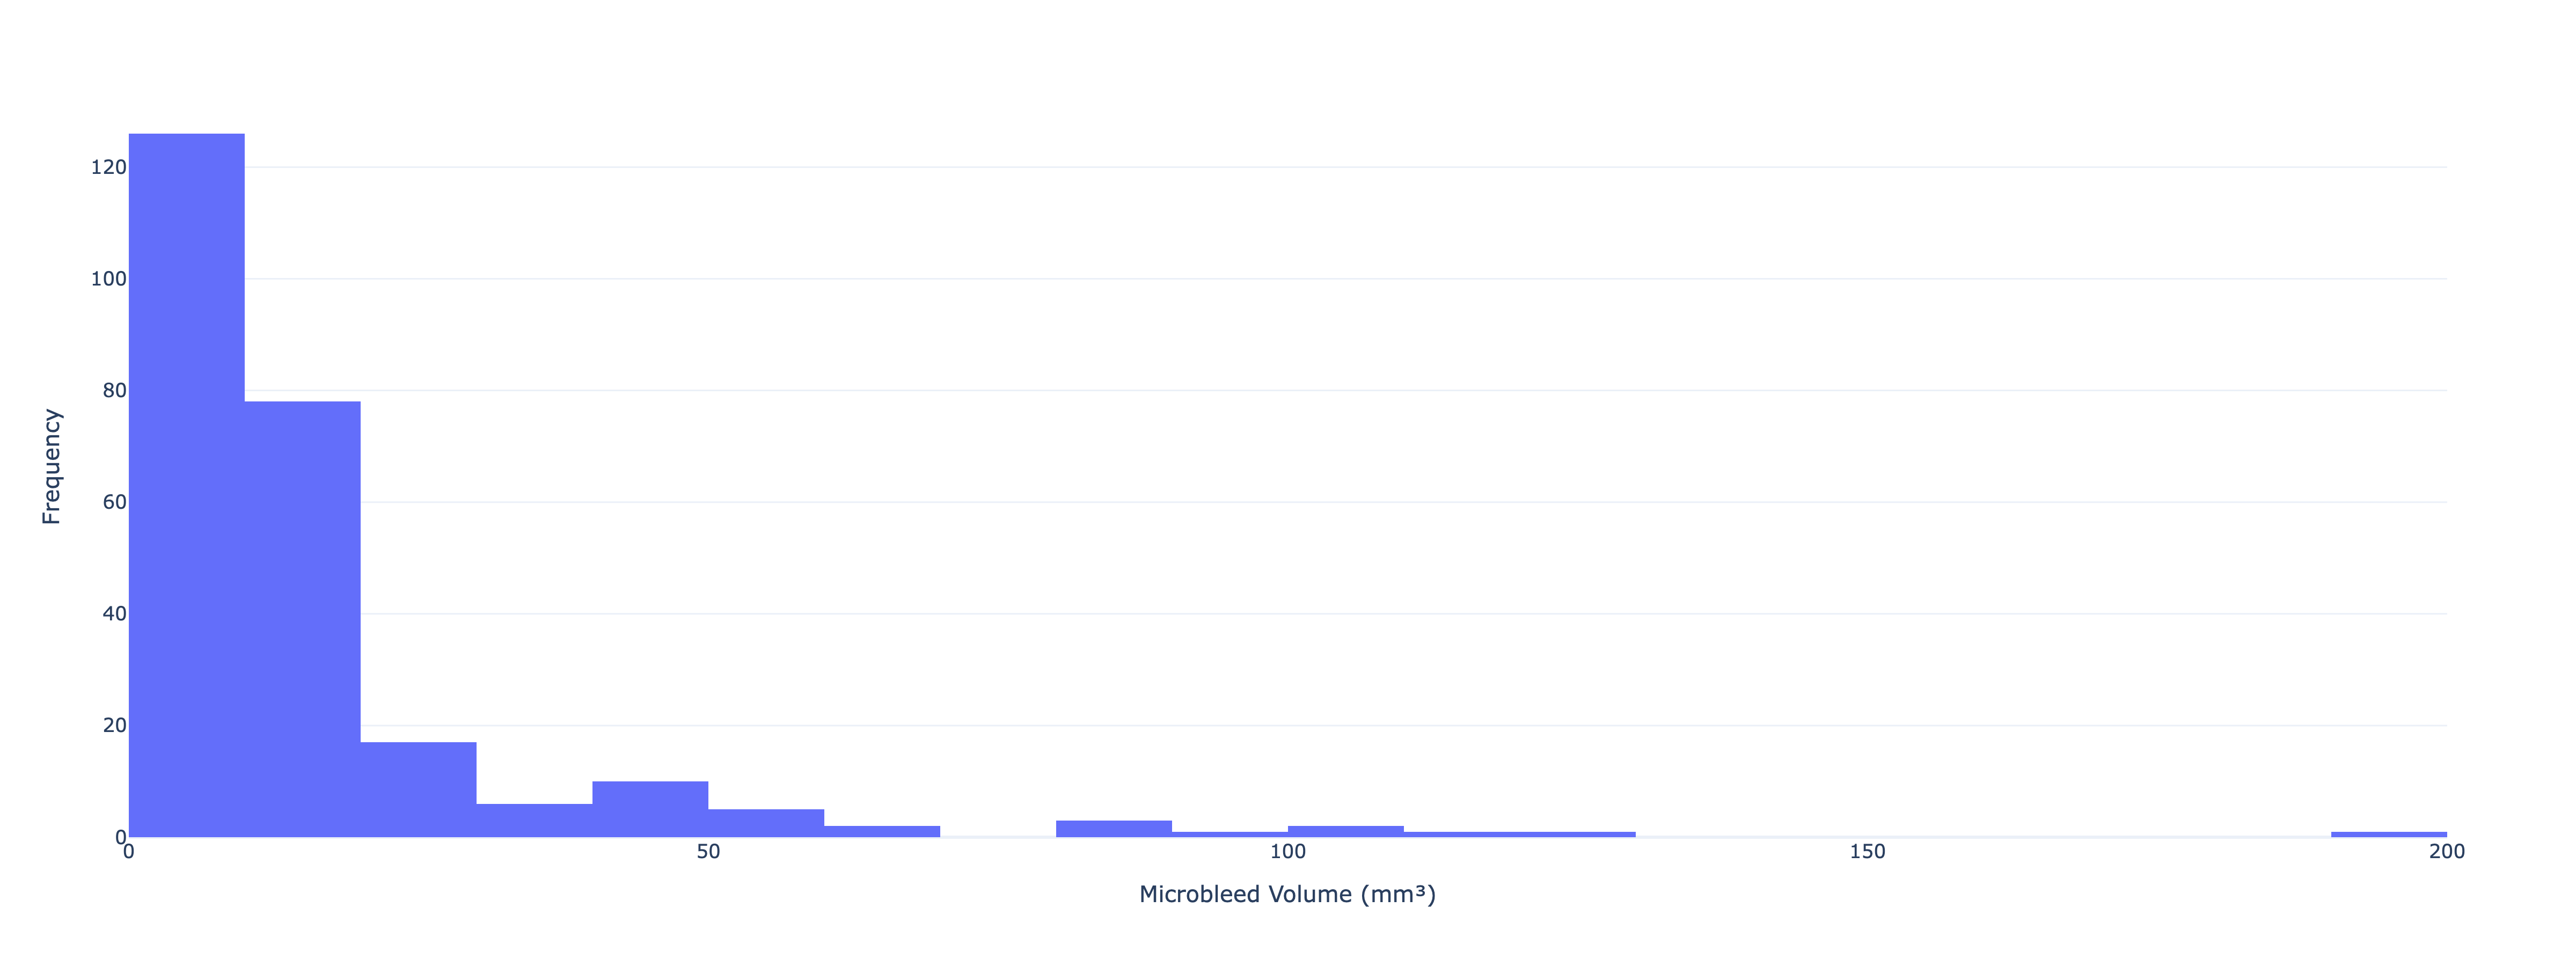
\includegraphics[width=0.75\textwidth]{cmb_vol_distr.png} 
    \caption{Histogram of individual microbleed sizes (in $mm^3$)}
    \label{fig:mb_sizes}
\end{figure}

\pagebreak

\section{Shared Baseline Pipeline}
\subsection{Methodology}

The methodology for this project is divided into two primary sections. The first section concerns the baseline model using the nnU-Net framework to perform automated detection of cerebral microbleeds, alongside an evaluation pipeline to extract custom evaluation metrics from the model inference stage. The second part, which is the individual contribution to this project, focuses on the development of an Interactive Exploration Dashboard to enable visual interaction with each subject and to analyse and interpret the model's outputs.
\\

Figure \ref{fig:system_architecture} illustrates the architecture of the completed pipeline, divided into three stages. The first stage is the preprocessing pipeline, which was described in detail in Section \ref{sec:dataset_stats}. The remaining stages correspond to the nnU-Net pipeline, encompassing the framework’s internal preprocessing, model training, and inference steps. The final stage is the Interactive Exploration Dashboard.

\begin{figure}[H]
    \centering
    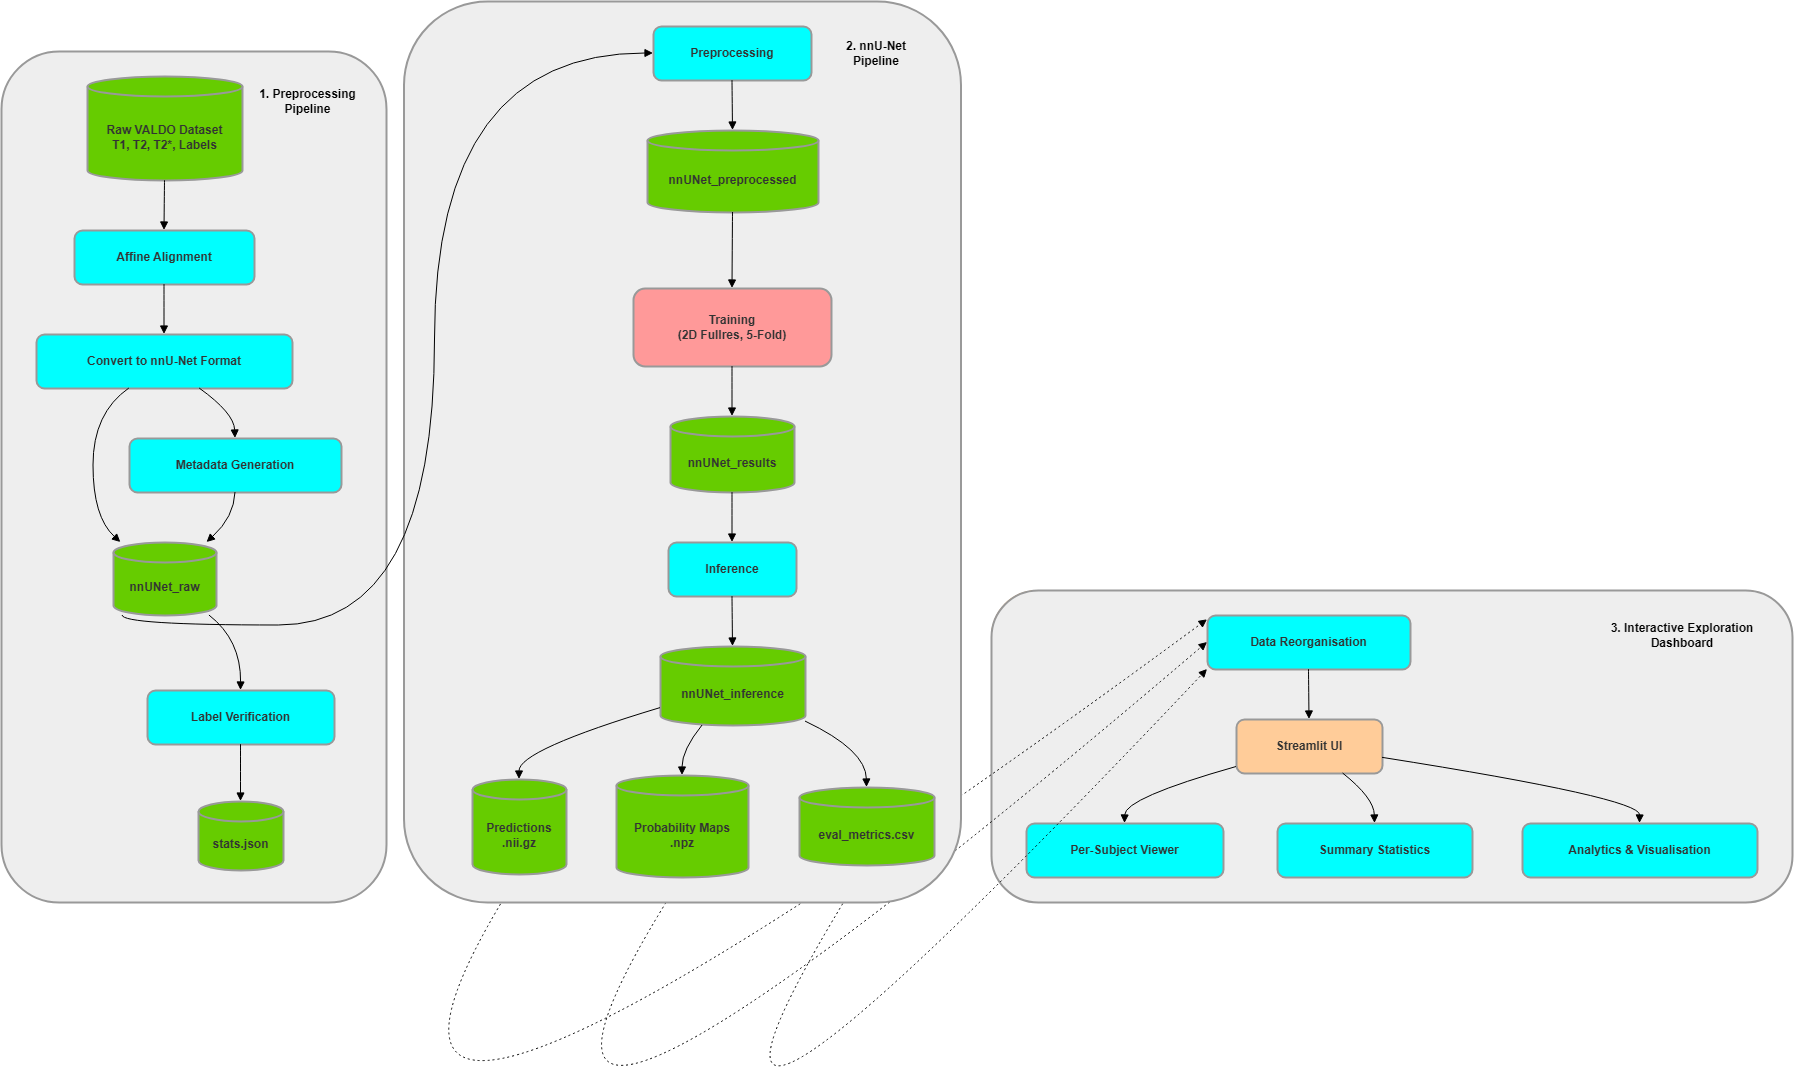
\includegraphics[width=\textwidth]{pipeline.png} 
    \caption{System architecture detailing the preprocessing pipeline, the nnU-Net framework processing stages, and the Interactive Exploration Dashboard.}
    \label{fig:system_architecture}
\end{figure}

\subsubsection{Baseline Model Training}
To establish a robust and reproducible baseline for microbleed detection, the nnU-Net deep learning framework was implemented \cite{nnUNet}. Since training was performed on three weighted volumes (T1, T2, $T2^*$) alongside segmentation masks of MRI slices, the task of cerebral microbleed detection is computationally expensive. For this reason, the 3D full-resolution configuration of nnU-Net was avoided, as it would significantly increase training time. Instead, the 2D full-resolution configuration was selected as a practical alternative, expected to achieve strong results with minimal performance loss despite the lack of inter-slice contextual information.
\\

To ensure the generalizability of the model and rigorously evaluate its performance on unseen data, a five-fold cross-validation strategy was applied to the VALDO training dataset. To ensure a reliable shared baseline was kept, the standard nnU-Net data splits were performed.

\subsubsection{Inference and Standardised Output Generation}
Once the nnU-Net model was trained, an inference pipeline was executed to generate predictions on the dataset. To ensure compatibility with the interactive dashboard, the outputs were standardised into three specific formats:
\begin{enumerate}
    \item \textbf{Prediction Masks}: NIfTI files (\texttt{.nii.gz}), one per subject, with the same case identifier as the original dataset. Binary segmentation masks (0/1) at the default nnU-Net threshold.
    \item \textbf{Probability Maps}: NumPy array files (\texttt{.npz}) containing the raw softmax confidence probabilities for the microbleed class, enabling dynamic thresholding for the interactive dashboard.
    \item \textbf{Evaluation Metrics}: A structured CSV file (\texttt{evaluation\_results.csv}) containing the quantified performance metrics per subject.
\end{enumerate}

\subsubsection{Evaluation Logic and Connected-Component Analysis}
\label{ss:eval}
Because microbleeds are sparse phenomena, relying solely on standard voxel-wise metrics (such as the Dice coefficient) can be misleading, as even a single misplaced voxel can significantly skew the score for very small objects. To address this, an evaluation script was developed to perform lesion-level connected-component analysis.
\\

The lesion-level evaluation was implemented as a per-subject analysis, where each ground-truth label is matched with its corresponding predicted mask. Both volumes were loaded and binarized, followed by 3D connected-component analysis using a $3\times3\times3$ connectivity structure to isolate individual microbleeds. A many-to-one overlap strategy was adopted such that ground-truth components overlapping with any predicted voxels were counted as True Positives, while predicted components with no overlap were classified as False Positives, and missed ground-truth components as False Negatives. Lesion-level sensitivity and precision were computed from these counts, with the F1-score defined as the harmonic mean of these values. In parallel, a voxel-wise Dice coefficient was calculated to quantify spatial overlap. This process was applied across all subjects and was exported as a per-subject CSV file for later analysis and visualisation.
\\

The following list of metrics is what what recorded during the evaluation process:

\begin{itemize}
    \item \textbf{Lesion-Level Sensitivity (Recall)}: This measures the proportion of actual microbleeds successfully identified by the model. A microbleed is considered a True Positive ($TP$) if the predicted mask overlaps the ground-truth microbleed by at least one voxel. Missed microbleeds are False Negatives ($FN$).
    \begin{equation}
        Sensitivity = \frac{TP}{TP + FN}
    \end{equation}
    
    \item \textbf{False Positives per Subject}: Number of incorrectly detected microbleeds by the model. A microbleed is considered to be a false positive if its corresponding connected component in the predicted mask has no spatial overlap with any ground-truth microbleed.

    \item \textbf{Lesion-Level F1-Score}: The F1-score provides us with a haromonic mean between the lesion-level precision and sensitivity, serving as a very strong metric to get the overall performance of the model within one value.
    \begin{equation}
        F1 = 2 \times \frac{Precision \times Sensitivity}{Precision + Sensitivity}
    \end{equation}

    \item \textbf{Voxel-Level Dice Coefficient}: While the above metrics evaluate performance at the object level, the Dice similarity coefficient evaluates the exact spatial overlap at the voxel level. Let $X$ be the set of ground-truth voxels and $Y$ be the set of predicted voxels:
    \begin{equation}
        Dice = \frac{2 |X \cap Y|}{|X| + |Y|}
    \end{equation}

    \item \textbf{Number of Ground Truth Microbleeds}: Total number of ground truth microbleeds for a given subject.
    
    \item \textbf{Number of Predicted Microbleeds}: Total number of predicted microbleeds by the model for a given subject.
\end{itemize}

\subsection{Results}

\subsubsection{Baseline Results}

The evaluation of the baseline nnU-Net model using the VALDO dataset shows very promising results, especially in terms of precision. As illustrated in the scatter plot Figure \ref{fig:scatter}, there is a significant positive correlation between the ground-truth microbleed counts and the predicted counts. The model displays exceptional accuracy for subjects with low microbleed counts. However, for severe cases
, such as for subject VALDO\_110, which contained 73 ground-truth microbleeds, the model exhibits a slight tendency to have a higher false negative count, resulting in a marginally lower sensitivity for extreme cases, but still manages to capture the majority of the bleeds.

\begin{figure}[H]
    \centering
    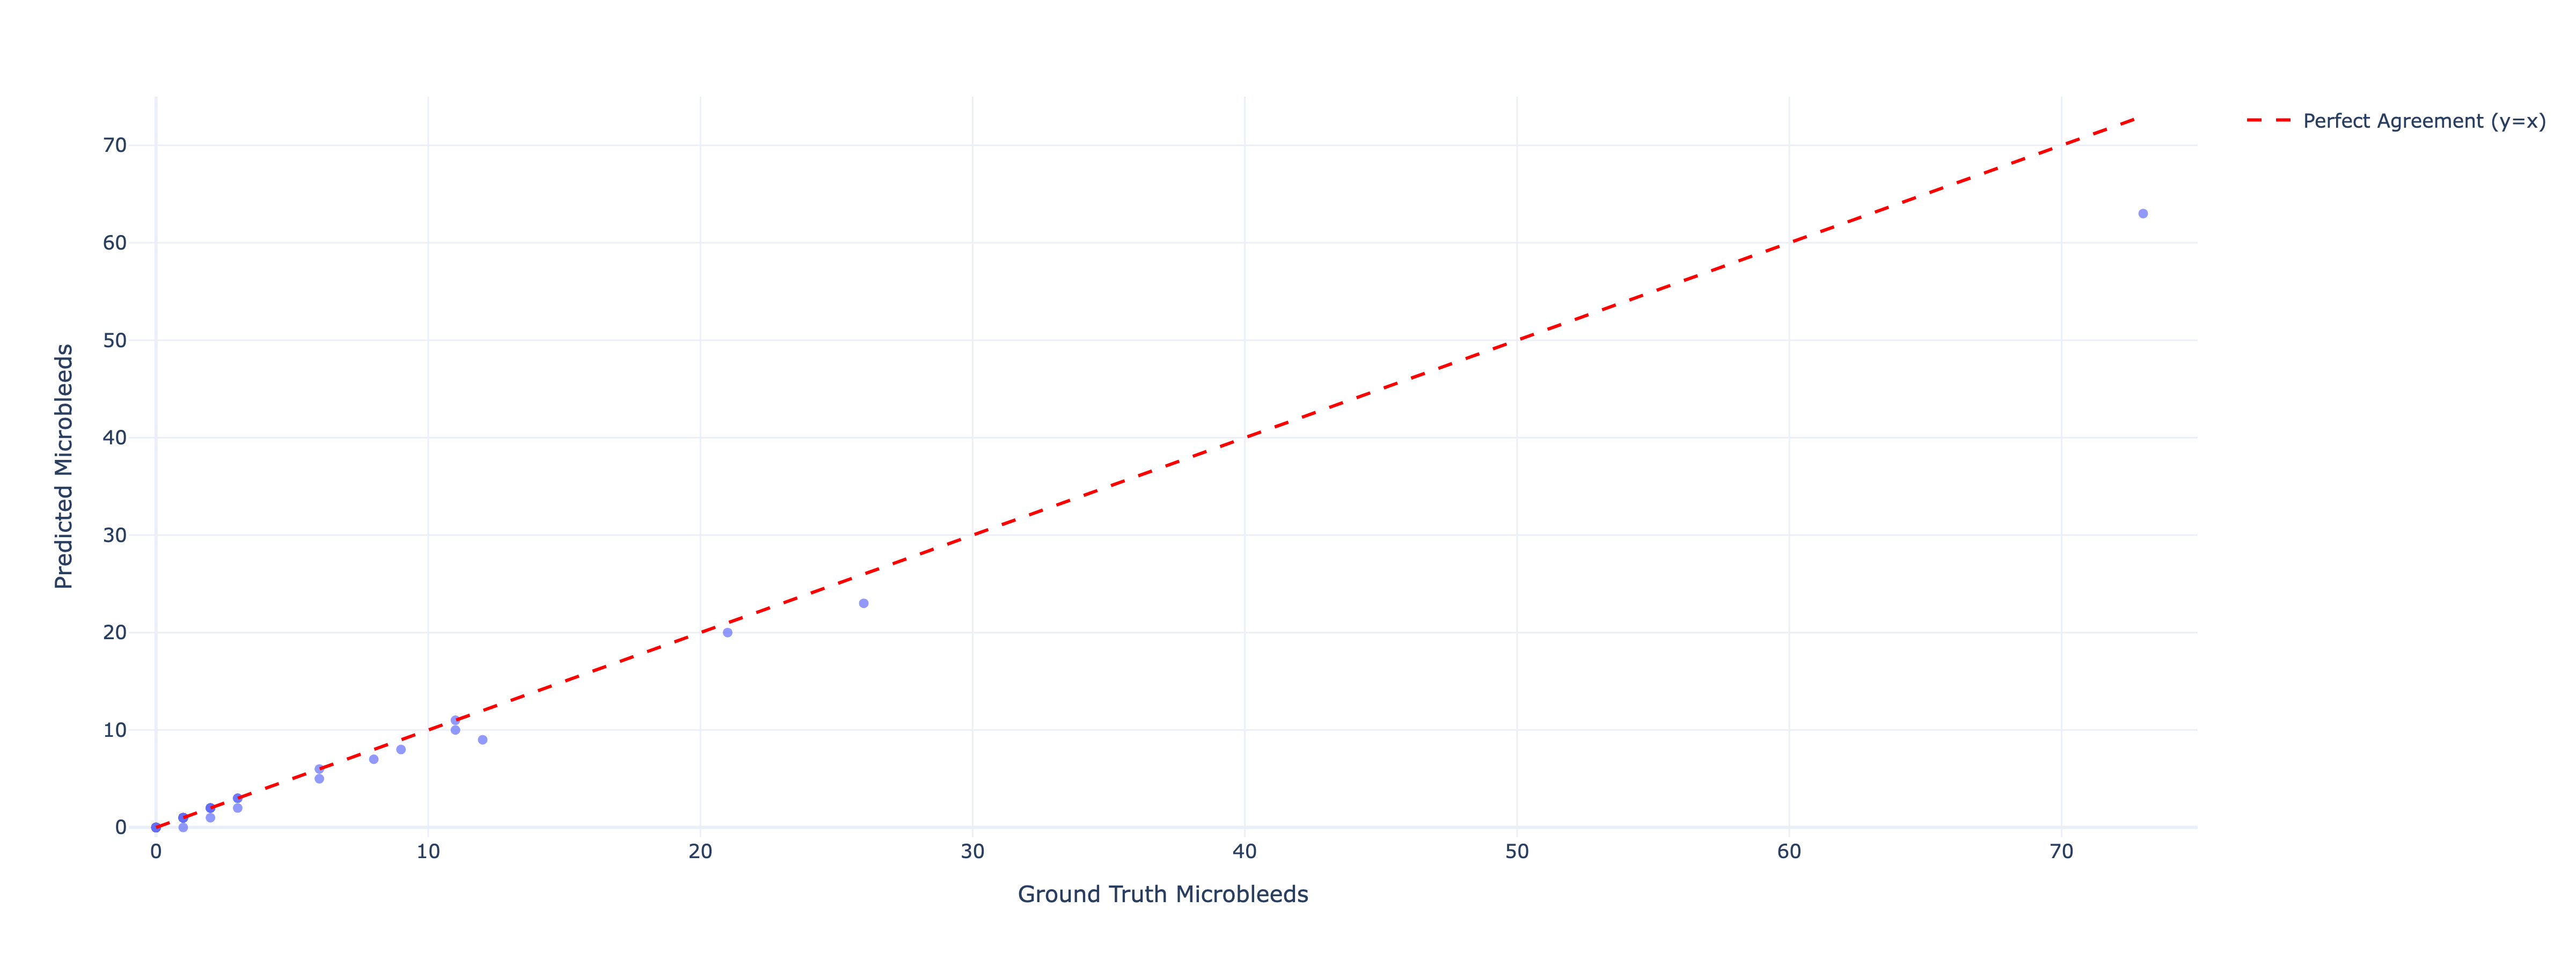
\includegraphics[width=\textwidth]{gt_pred_scatter.png} 
    \caption{Scatter plot of Ground Truth vs. Predicted Microbleed Counts per Subject.}
    \label{fig:scatter}
\end{figure}

Taking a closer look at the performance of the model, as presented in the boxplot Figure \ref{fig:boxplot}, we can get a stronger idea of where our model lies. The median values for Lesion-Level Sensitivity, F1-Score, and the Voxel-Level Dice Coefficient are all concentrated near 1.0. One of the most interesting observations that was made has to do with the False Positive rate, which was negligible across all evaluated subjects. The most volatile metric was the Dice coefficient, which is mathematically expected as a single misclassified voxel significantly penalises the spatial overlap metric for tiny structures like cerebral microbleeds, even if the lesion was successfully detected at the object level.

\begin{figure}[H]
    \centering
    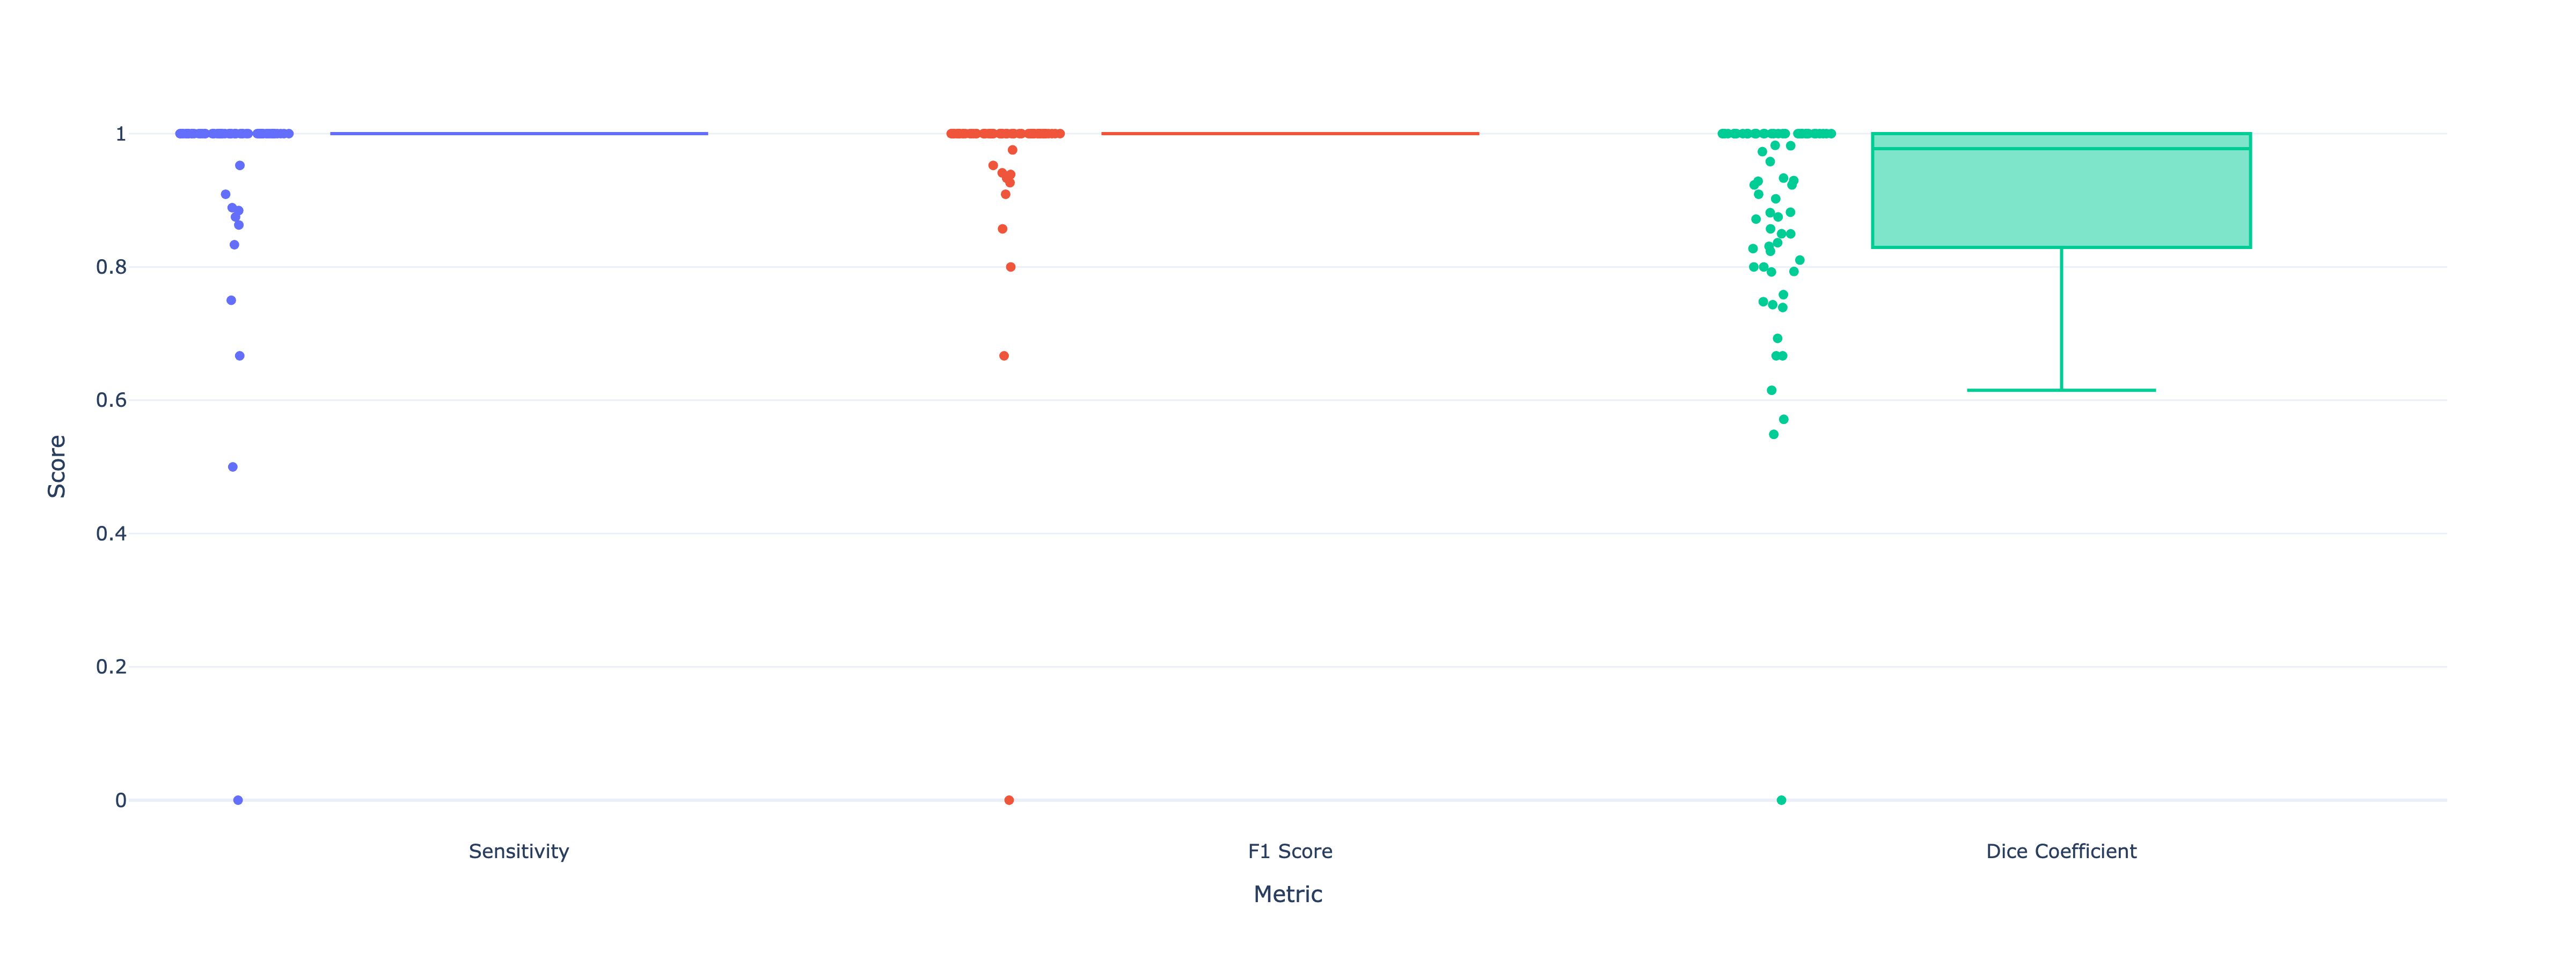
\includegraphics[width=1\textwidth]{eval_metrics_boxplot.png}
    \caption{Boxplot distribution of Lesion-Level Sensitivity, F1-Score, and Voxel-Level Dice Coefficient across all subjects.}
    \label{fig:boxplot}
\end{figure}

\subsubsection{Aggregate Performance Statistics}

To quantify the model's performance across the entire dataset of 72 subjects, we can view the statistical summary table found in Table \ref{tab:summary_stats}. The most remarkable finding from Table \ref{tab:summary_stats} is that the model produced zero false positives across all subjects, resulting in perfect precision.

Both Sensitivity and the F1-Score achieved a median of 1.000, indicating a perfect lesion-level detection for the majority of the dataset. The mean Sensitivity (0.960), mean F1-Score (0.971) and mean Dice coefficient (0.895) are just slightly lower than their respective medians, indicating that the place where the model suffered most was at the rare edge cases where the model failed to detect highly clustered or exceptionally small microbleeds.

\begin{table}[H]
    \centering
    \begin{tabular}{l c c c c c}
        \hline
        \textbf{Metric} & \textbf{Mean} & \textbf{Std. Dev.} & \textbf{Min} & \textbf{Median} & \textbf{Max} \\
        \hline
        Sensitivity & 0.960 & 0.141 & 0.000 & 1.000 & 1.000 \\
        F1-Score & 0.971 & 0.127 & 0.000 & 1.000 & 1.000 \\
        Dice Coefficient & 0.895 & 0.160 & 0.000 & 0.977 & 1.000 \\
        Ground-Truth Microbleeds & 3.28 & 9.46 & 0 & 1 & 73 \\
        Predicted Microbleeds & 2.94 & 8.24 & 0 & 1 & 63 \\
        \hline
    \end{tabular}
    \vspace{0.2cm}
    \caption{Summary statistics of model performance across all 72 subjects.}
    \label{tab:summary_stats}
\end{table}

\FloatBarrier
\clearpage

\section{Individual Research Thread: Interactive Exploration Dashboard}
\subsection{Methodology}
To bridge the gap between aggregate statistical metrics and qualitative spatial analysis, an Interactive Exploration Dashboard was developed. The core aim of this research thread is to provide researchers and clinicians with an interface to inspect individual test subjects slice-by-slice. Furthermore, it allows users to visually evaluate the model's predictions and observe how dynamic adjustments to the probability threshold directly impact the network's predictive capabilities.
\\

The application was built using a modular architecture in Python. The data ingestion pipeline, managed via a \textbf{reorganisation} script, automatically extracts the NIfTI MRI volumes, binary masks, raw softmax probability maps and the evaluation summary from the nnU-Net inference outputs and resturctures them in the accepted format for the interface.  Figure \ref{fig:system_architecture}
\\

The backend processing relies heavily on \textbf{NiBabel} for managing neuroimaging data. A custom NIfTI loader extracts the 3D voxel arrays alongside their affine matrices to ensure accurate spatial orientation. To evaluate performance at the lesion level, a connected-component matching algorithm was constructed and follows a similar implementation to that in Section \ref{ss:eval} to ensure accurate calculations throughout the entire project. The algorithm extracts distinct components from the prediction masks and evaluates their spatial intersection with ground-truth components to classify each prediction dynamically.
\\

The frontend user interface was developed using the \textbf{Streamlit} framework, chosen for its implementation simplicity and modern features. The dashboard is split into three views, the per subject slice viewer, a dataset summary section and graph analysis.

\subsubsection{Per-Subject Slice Viewer}
\label{ss:per_sub_view}
The core component of the dashboard is a multi-planar slice navigation interface, allowing users to traverse the 3D MRI volume across the axial, sagittal, and coronal planes. To aid qualitative analysis, segmentation masks are rendered as colour-coded overlays directly on top of the rendered slice, with true positives shown in green, false positives in red, and false negatives in yellow.
\\

A key feature implemented within this viewer is the \textbf{dynamic probability thresholding}. Using a threshold slider ranging from 0.0 to 1.0, users can dynamically adjust the threshold applied to the raw softmax probability maps. Updating this threshold triggers a real-time recalculation of the connected components, instantly refreshing the overlay visualisations. Users are also able to toggle the segmentation masks on and off to directly compare the model's predicted segmentations against the underlying microbleeds.
\\

To further connect these spatial visualisations with quantitative evaluation, a dedicated metrics section is displayed alongside the slice viewer. This section holds subject-level detection statistics, including the counts of true positives, false positives, and false negatives, as well as the total number of ground-truth and predicted microbleeds. Additionally, the performance metrics (sensitivity, precision, and F1-score) are also included. An important note is that each of these metrics are immediatly updated the second you adjust the probability threshold to give a dynamic experience of the interface.

\subsubsection{Dataset Summary and Analytics}
\label{ss:dataset_summ_analytics}
The remaining two sections focus on the analytical components of the interface.
\\

The macro-level analysis is presented within the \textbf{Dataset Summary} section, where an interactive dataframe was added to display the evaluation metrics for all subjects, including F1-score, sensitivity, Dice coefficient, false positives, ground-truth counts, and predicted counts. Alongside this table, an evaluation overview was included to provide aggregated statistics for the key metrics, namely F1-score, sensitivity, Dice coefficient, and false positives. Additionally, a key feature was implemented where users can also select a subject directly from the interactive table, and it will automatically update the per-subject viewer to display the corresponding scans and predictions.
\\

The visual analysis component is presented in the \textbf{Graph Analysis} section, where two dynamic charts were implemented using Streamlit's charting libraries: the microbleed count per subject and the sorted F1-score per subject.
\\

The first chart provides a frequency distribution of the ground-truth microbleeds across all inference subjects. This visualisation was mainly added to highlight class imbalances within the dataset.
\\

The second chart plots the F1-score of each subject in ascending order. By sorting the data from worst to best performance, this chart allows the user to quickly interpret the model's overall consistency. The main purpose of this chart was to support the rapid identification of poorly performing subjects so that they could then be examined in greater depth in the \textbf{Dataset Summary} and \textbf{Per-Subject Viewer} sections.

\subsection{Results}
\label{ss:results_dashboard}

The integtation of the Interactive Exploration Dashboard to the validation allowed for the transformation of the evaluation process from a static statistical summary into a dynamic and clinically interpretable diagnostic review. While the aggregate metrics (shown in Table \ref{tab:summary_stats}) provide a meaningful high-level overview of model performance, they often fail to fully capture the sensitivity and complexity associated with CMB detection. By leveraging the dashboard’s architecture, a more human-interpretable analysis of the model’s predictive ability became possible, revealing subtle details in probability calibration and small-object localisation that were previously overlooked. The following section therefore discusses both qualitative and quantitive insights obtained through a more detailed inspection of the model's predictive performance.

\subsubsection{Qualitative Analysis: Per-Subject Slice Viewer Tab}
The per-subject viewer shown in Figure \ref{fig:per_sub_view} enabled a direct spatial verification of the model's detections against the ground-truth annotations. By implementing a real-time connected-component matching algorithm, the dashboard provided immediate visual feedback through color-coded prediction overlays.

\begin{figure}[H]
    \centering
    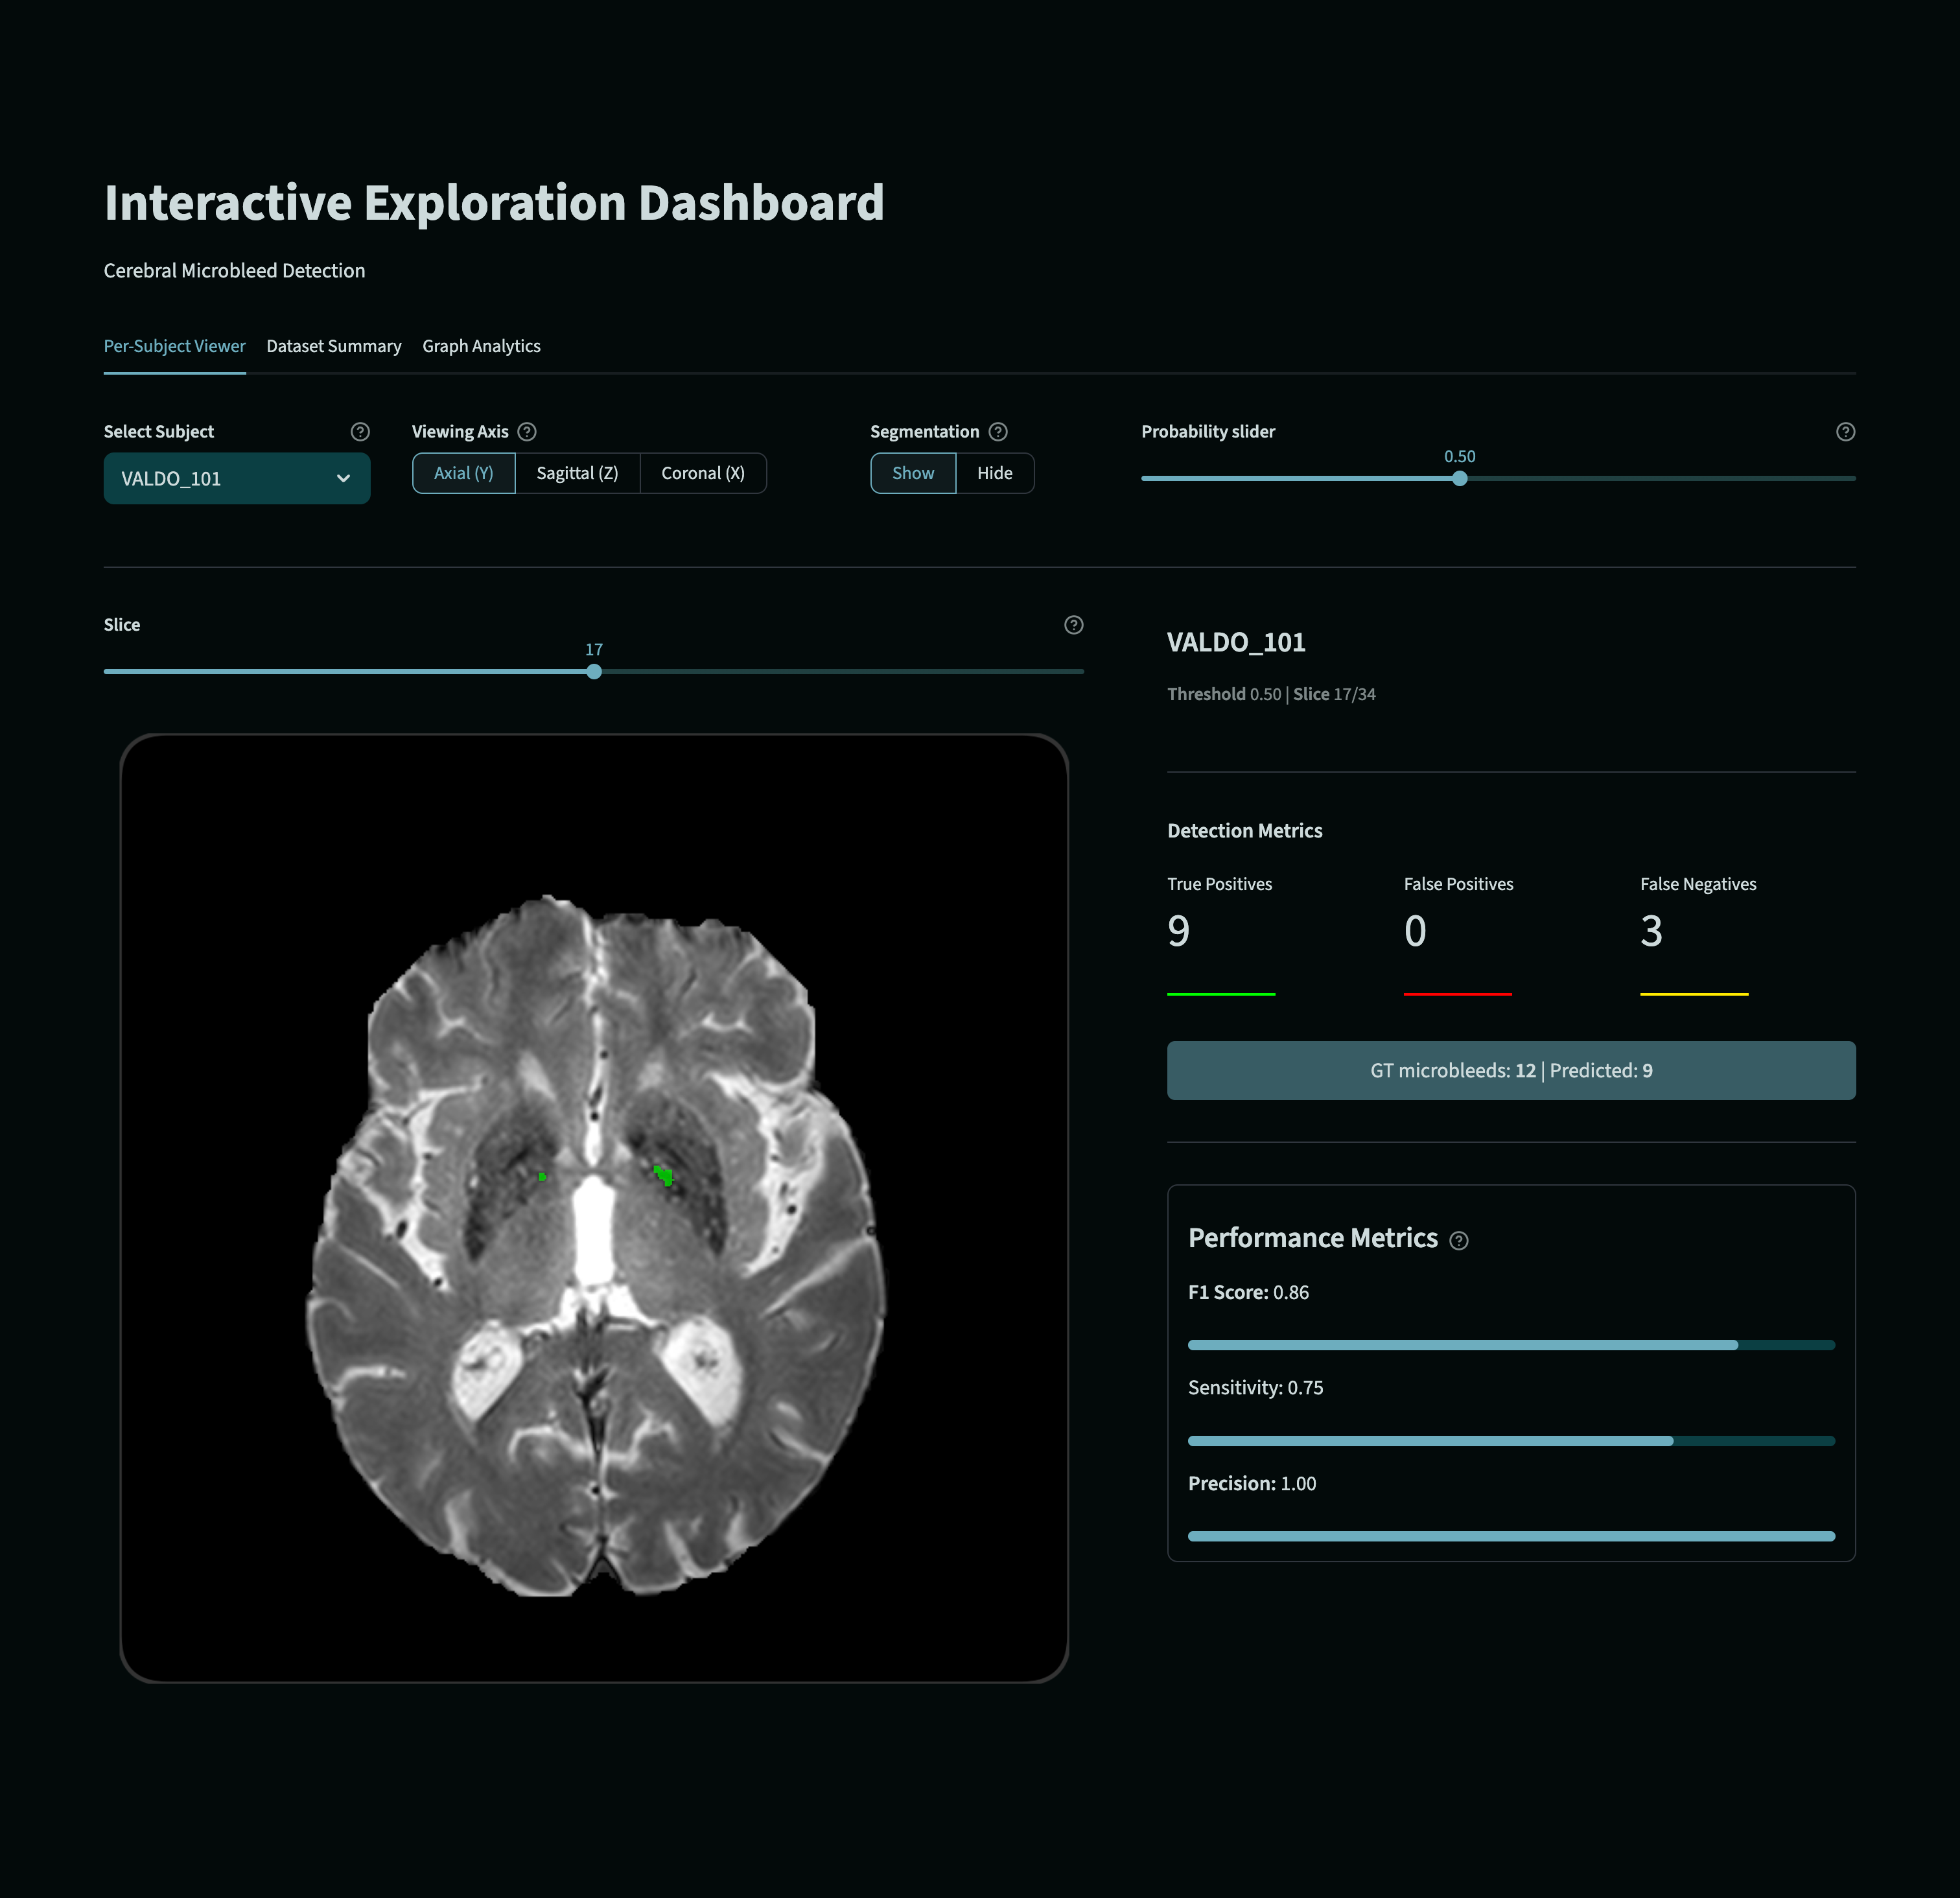
\includegraphics[width=0.8\textwidth]{per_sub_view.png}
    \caption{The Per-Subject Slice Viewer interface. In this instance, we hace subject VALDO\_101 at slice 17 with two correctly predicted lesions highlighed in green.}
    \label{fig:per_sub_view}
\end{figure}

A key finding facilitated by this tool was the observation of \textbf{sub-threshold localisation}. Through the use of the dynamic probability slider, it was discovered that the baseline model's False Negatives could be significantly reduced by simply setting the softmax probability threshold to be slightly less strict then the default of 0.5. This value, through empirical testing, was often in the range of  $P(x) \in [0.25, 0.40]$ where at these value from the subject viewer, the overlays of the False Negatives (yellow) are instantly convert to True Positives (green). This result suggests that what the model considers as failures are often a matter of probability calibration rather than the model failing to capture the necessary features, indicating that a slightly less strict threshold could be beneficial to the model performance without having the risk of higher false positive counts.

\subsubsection{Quantative Analysis: Dataset Summary Tab}
The dashboard's interactive performance table (Figure \ref{fig:data_summary}) was integrated with the main scope for triaging the validation subjects.

\begin{figure}[H]
    \centering
    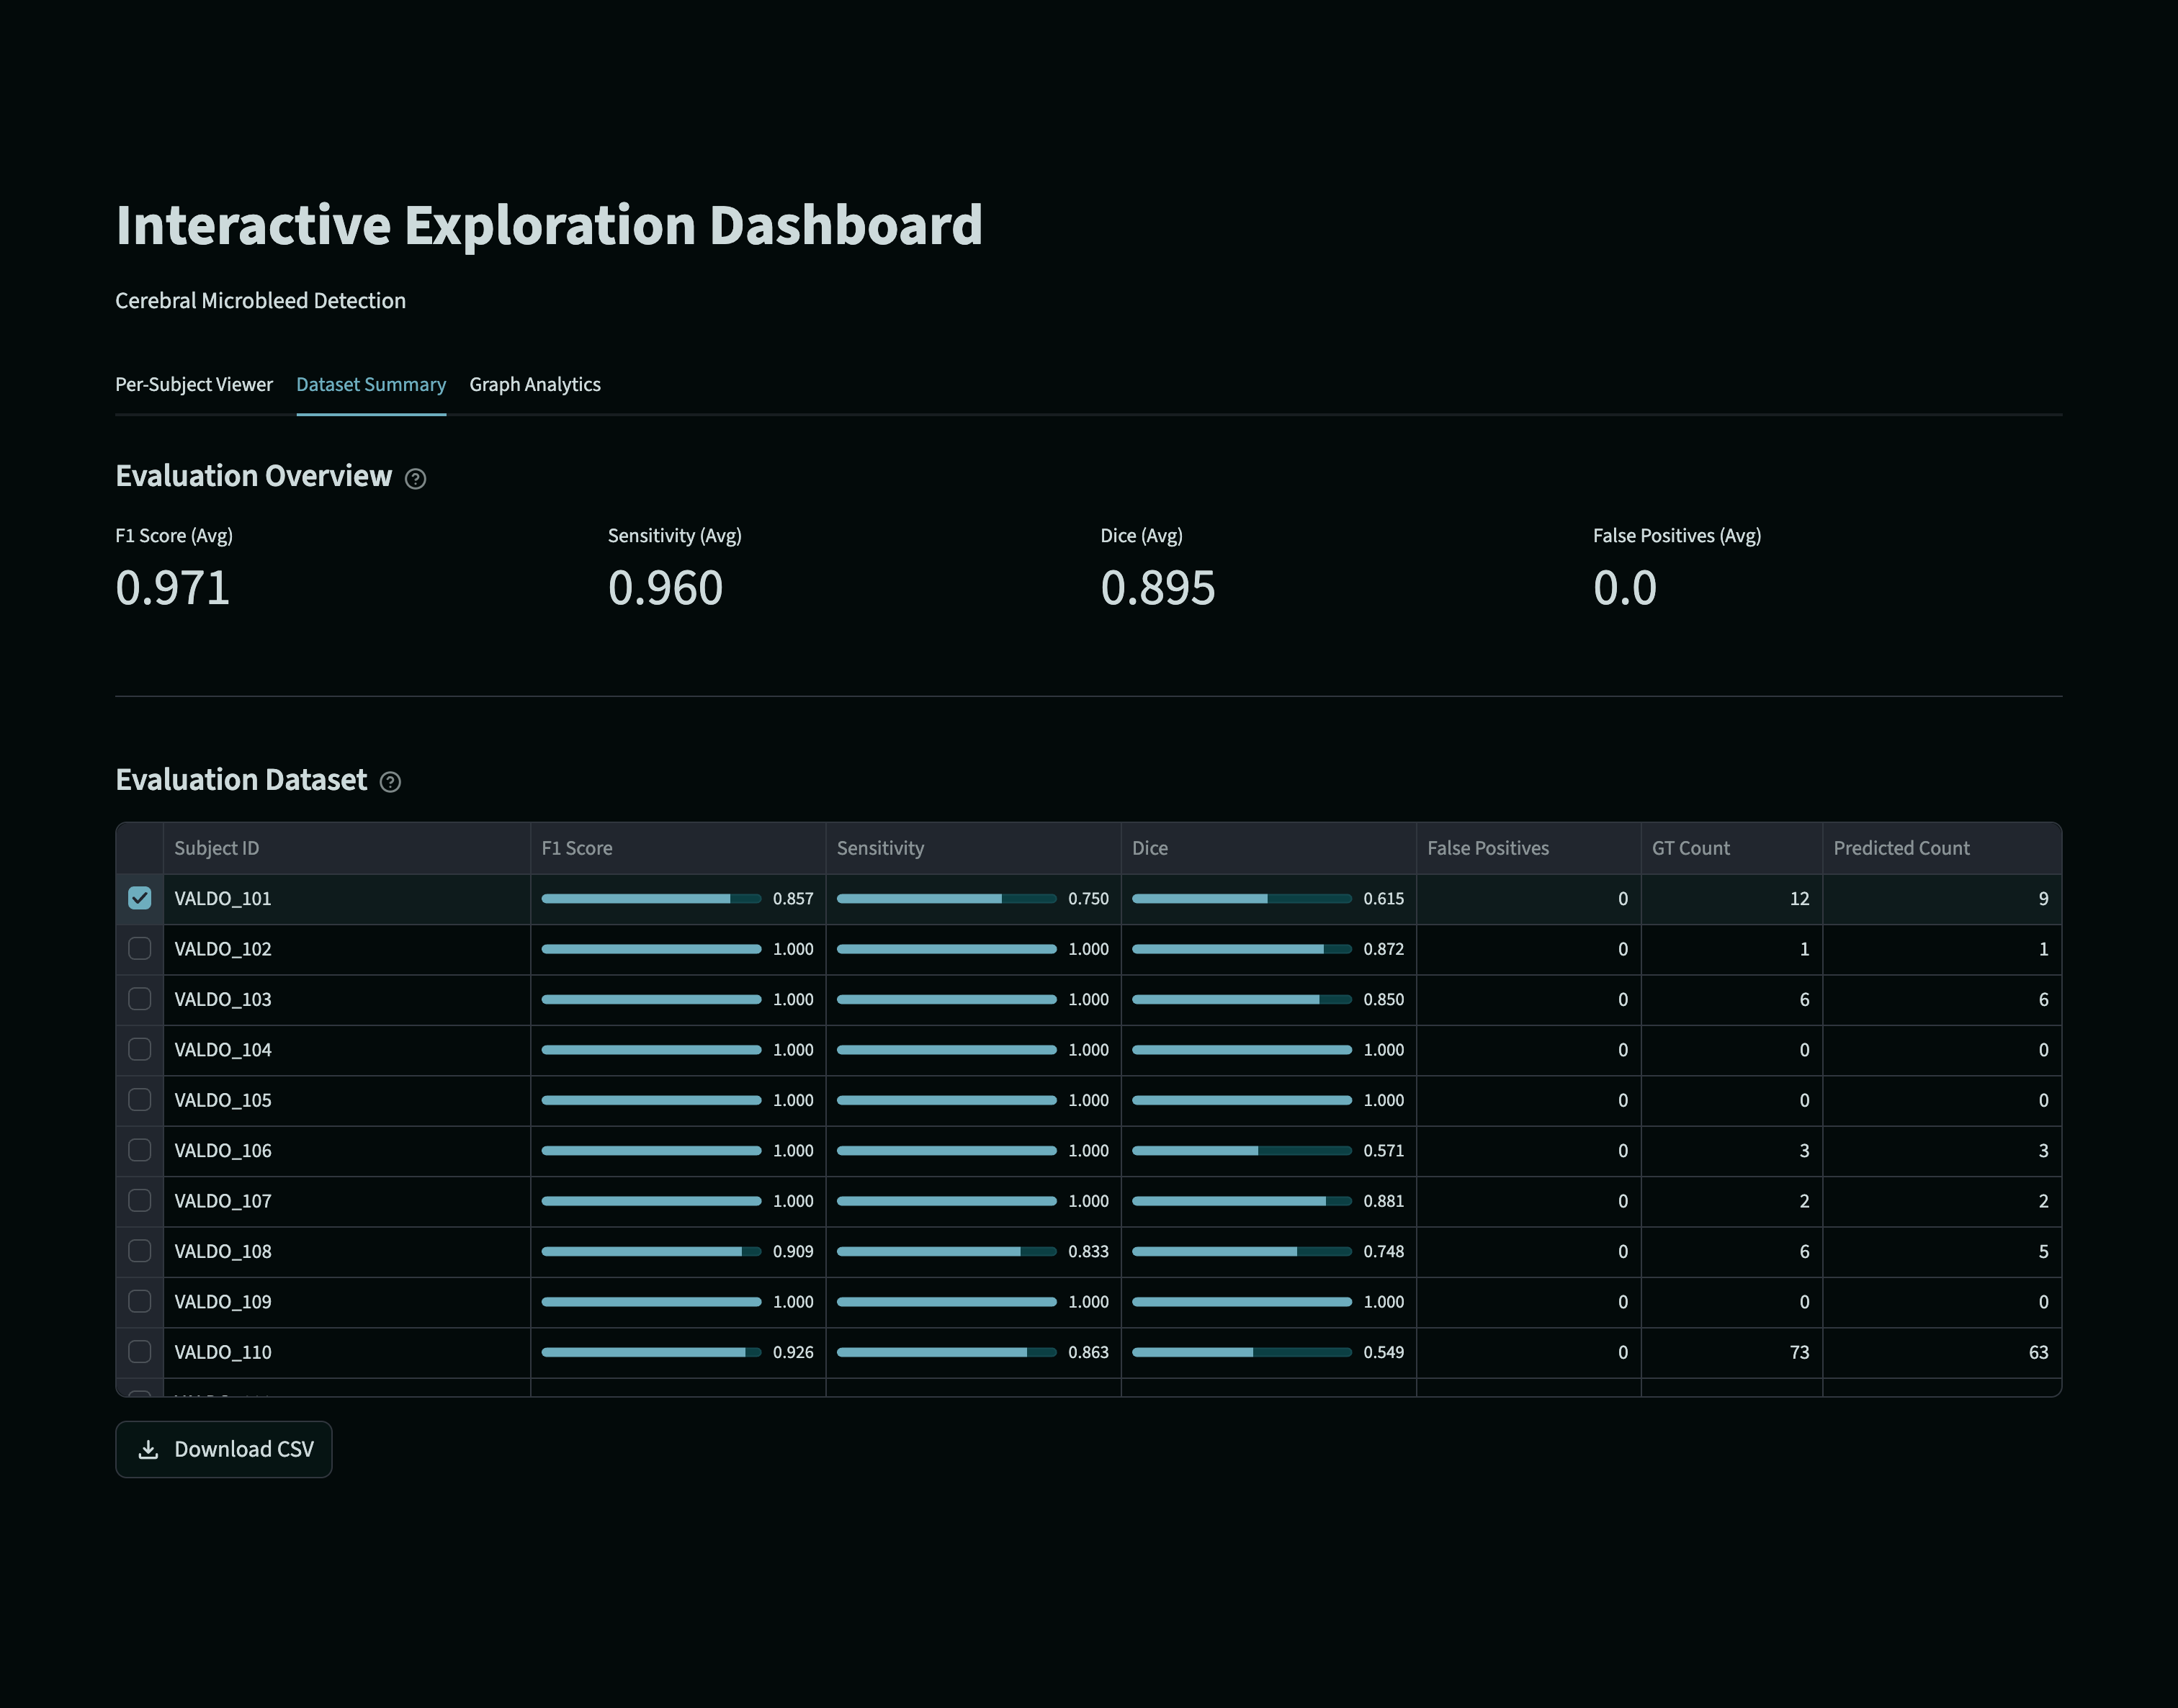
\includegraphics[width=0.8\textwidth]{data_summary.png}
    \caption{The Dataset Summary tab. Includes all key metrics for each subject and alows for sorting by any desired metric}
    \label{fig:data_summary}
    \rightfigure
\end{figure}

The facility of sorting subject by key metrics, such as F1-score and sensitivity allowed for quick identification of poor performing subjects. Specifcally, the Dataset Summary Tab indicated that the drop in performance 

The ability to sort subjects by F1-score and predicted count allowed for the rapid identification of failure modes. Specifically, the dashboard highlighted that performance drops were not random but were concentrated in subjects with either extremely small, single-voxel lesions or highly atypical lesion clusters. By isolating these cases in the table, the researcher could navigate directly to the problematic slices, saving significant manual search time compared to traditional NIfTI viewing tools.

\subsubsection{Macro-Level Statistical Analysis}
The automated graphical analysis (Figure \ref{fig:graph_analysis}) provided a macro-level perspective on the model's consistency across the varying distributions of the VALDO dataset.

\begin{figure}[H]
    \centering
    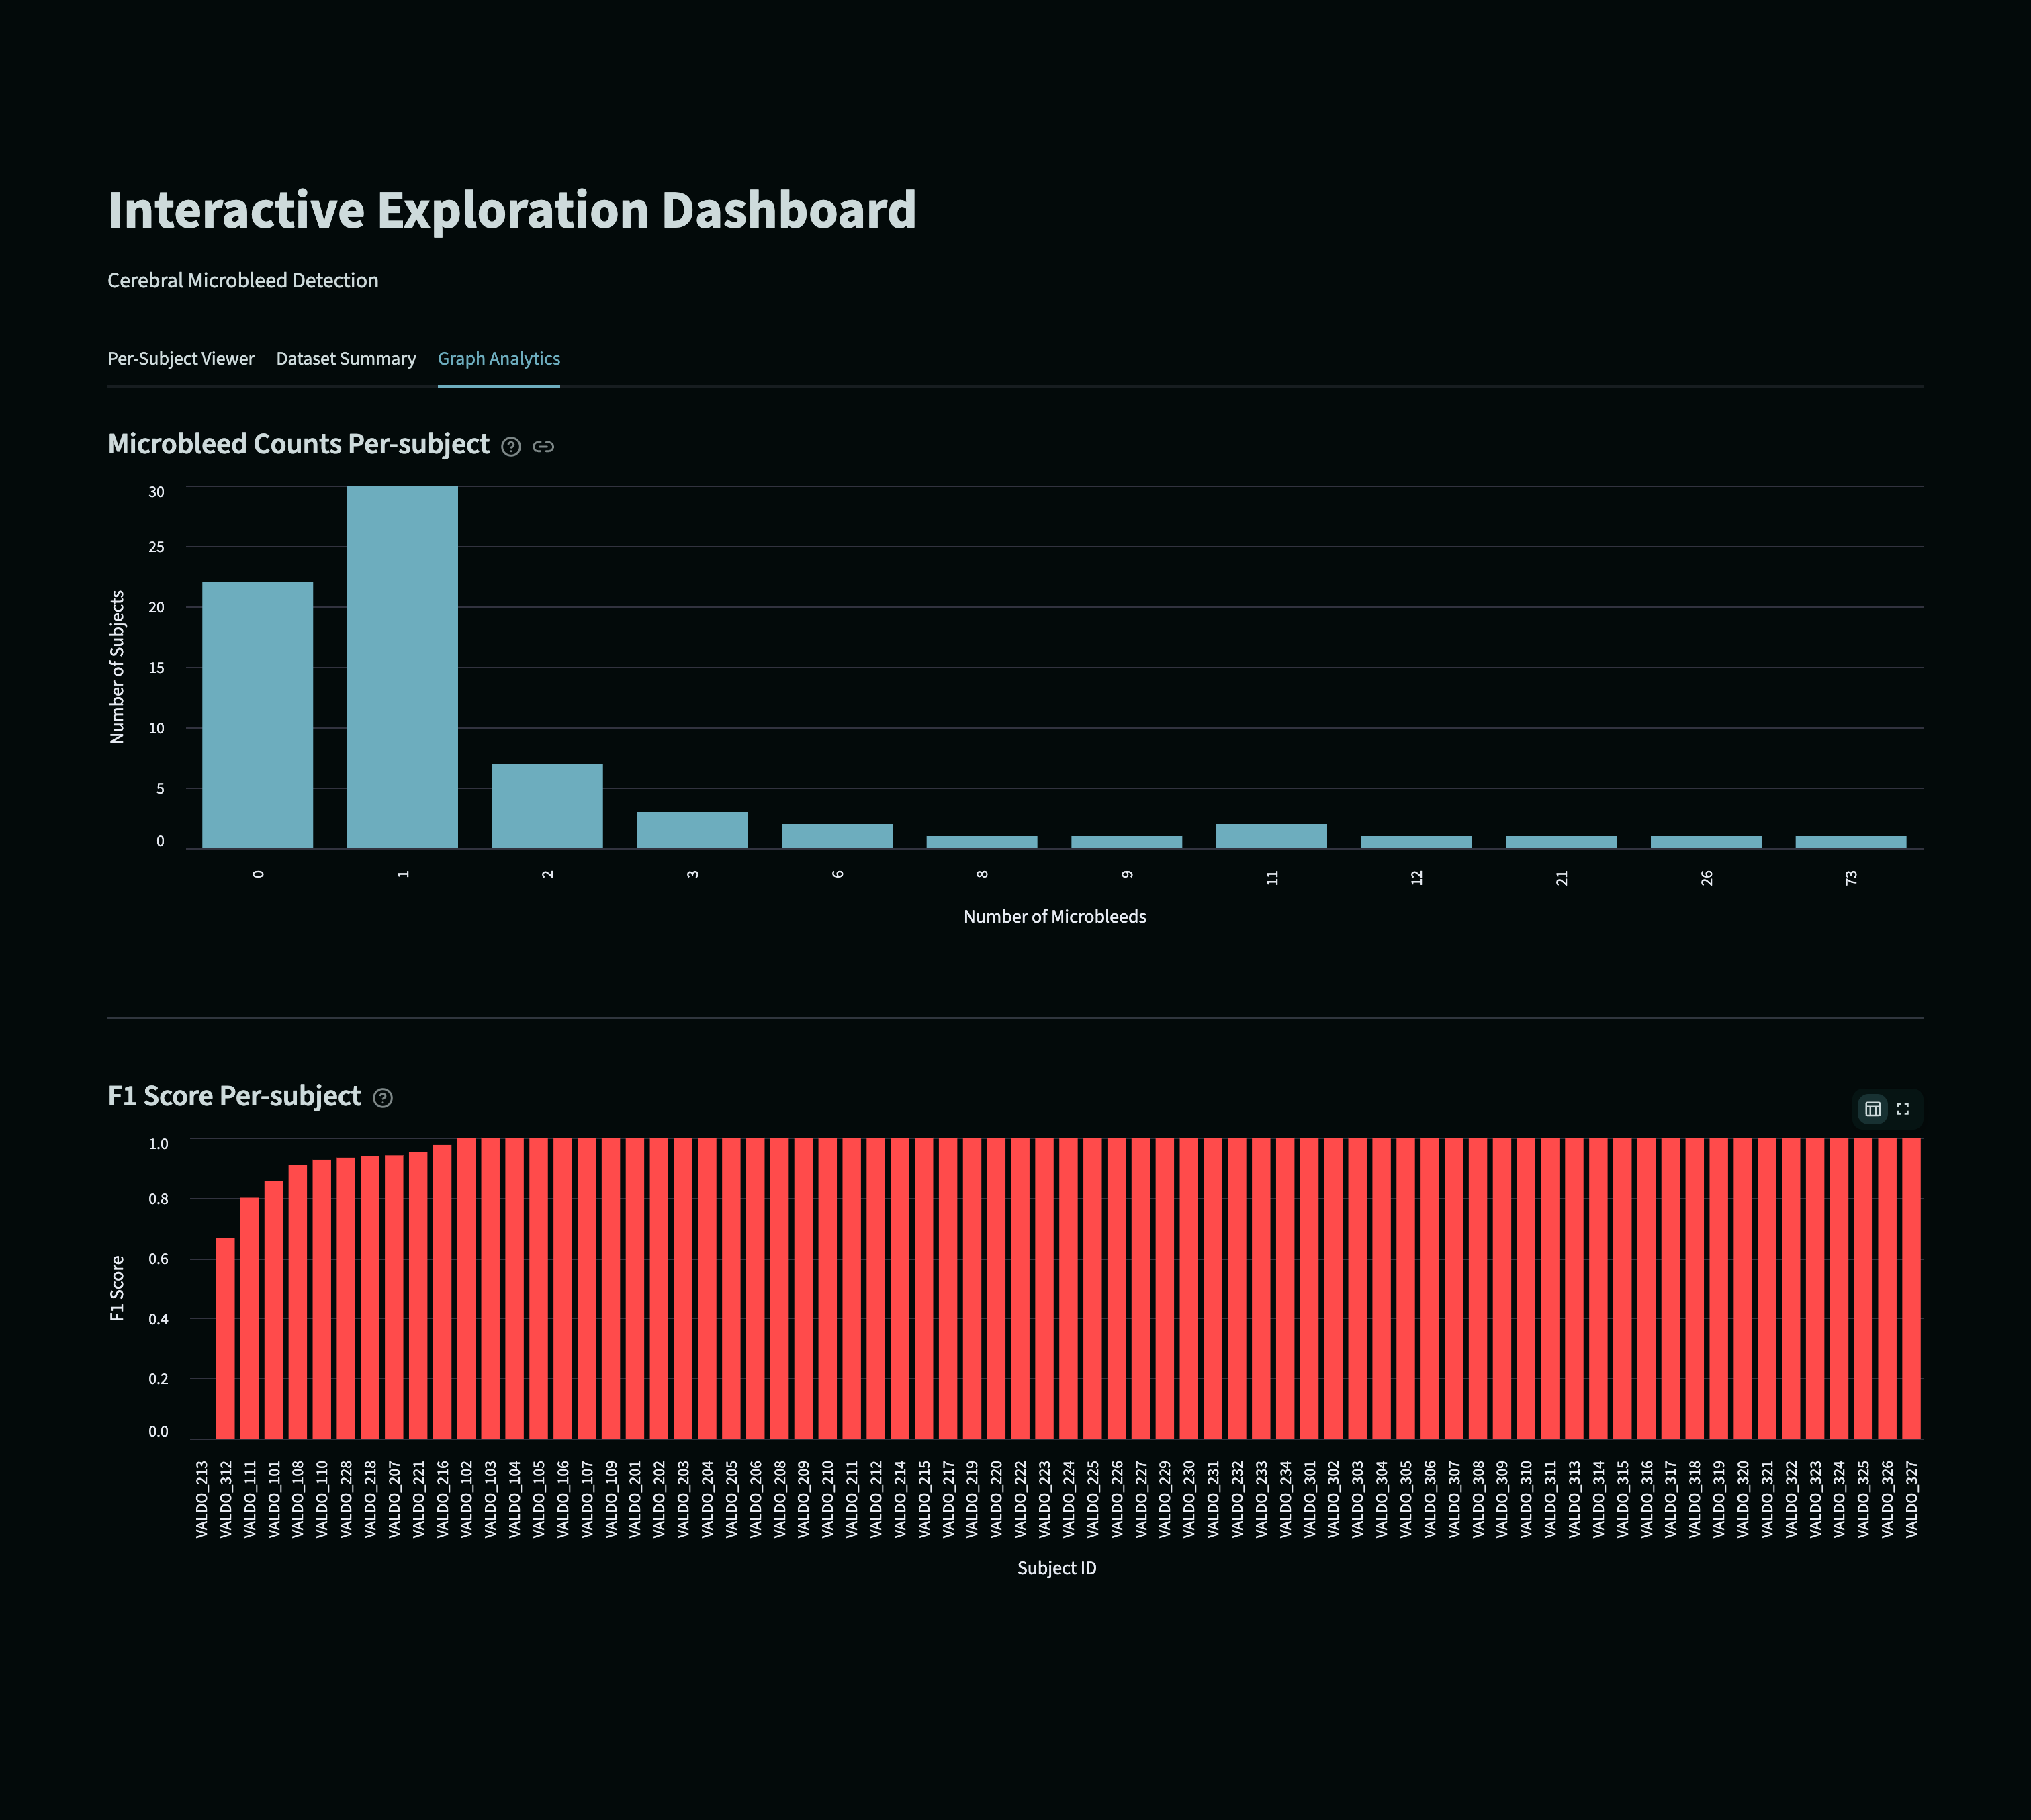
\includegraphics[width=0.8\textwidth]{graph_analysis.png}
    \caption{Automated graphical analysis of the dataset, illustrating the frequency distribution of ground-truth microbleeds (top) and an ordered ranking of per-subject F1-Scores (bottom).}
    \label{fig:graph_analysis}
\end{figure}

The distribution of microbleed counts (top chart) confirms a heavy "long-tail" distribution, where the majority of subjects present with zero to two lesions. The corresponding F1-score ranking (bottom chart) demonstrates that the model is exceptionally robust on these "standard" clinical cases, with over 75\% of the dataset achieving an F1-score of 1.0. The visual evidence confirms that the model's primary challenge lies not in general performance, but in the rare, high-burden outliers that occupy the lower end of the sorted F1 distribution.

\subsubsection{Summary of Utility}
Ultimately, the dashboard results demonstrate that for small-object detection tasks, voxel-wise metrics like Dice are insufficient for a complete evaluation. The tool provides the necessary evidence to show that even when a model's Dice score is mathematically penalized by the small size of the objects, its clinical localization is often highly accurate. This dual-view approach proves that interactive visual analytics are a mandatory companion to standard deep learning benchmarking, providing the transparency essential for building trust in AI diagnostic systems.

\section{Conclusions}

There is not much to conclude here.

\pagebreak


\nocite{*}

\bibliographystyle{plain}
\bibliography{refs}

\end{document}
